\section{Arbeitslosigkeit}
\subsection{Sockelarbeitslostigkeit \ho{Ho7}}
  Sockelarbeitslosigkeit entsteht wenn Arbeitskr�fte falsch ausgebildet sind. Es
  ist ein Zeichen f�r Strukturwandel. Derzeit gr�sster Wandelfaktor ist der
  starke Schweizer Franken / schwache Franken.\\
  Sockelarbeitslosigkeit entsteht nur bei stabilen L�hnen, gibts aber bei
  sinkenden L�hnen nicht. Die Arbeitskr�fte die bei sinkenden L�hnen nicht mehr
  arbeiten sind nicht Arbeitslos, da sie es freiwillig machen.
  \newpage
\subsection{Konjunktur und Arbeitslosigkeit \ho{Ho8}}
\begin{multicols}{2}
	\subsubsection{Makro�konomisches Grundmodell \ho{Ho8 F5}}
		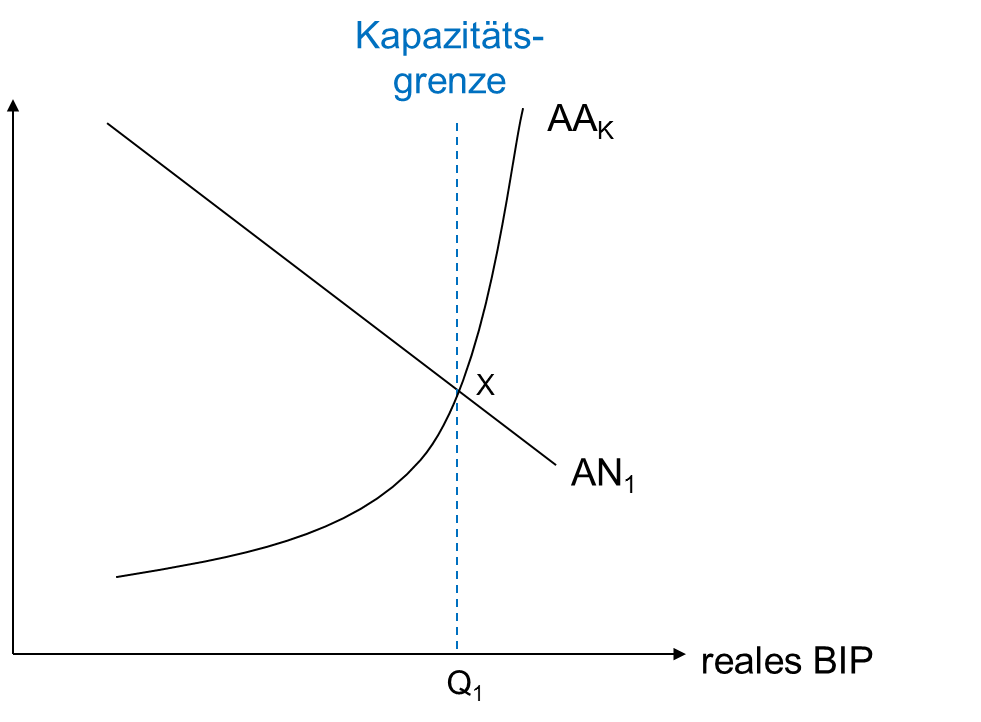
\includegraphics[width=9cm]{./bilder/h08f08.png}
	\subsubsection{Konjunkturelle Arbeitslosigkeit \ho{Ho8 F8FF}}
	  Entsteht durch einen Nachfrageschock und besteht nur kurzfristig.
			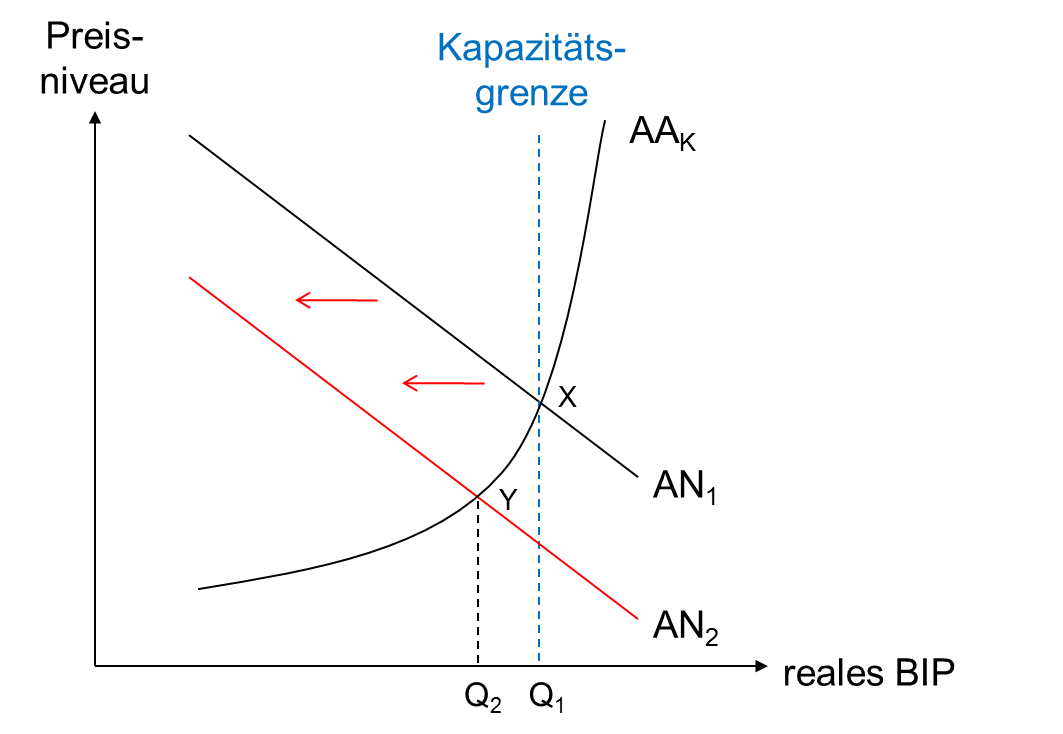
\includegraphics[width=9cm]{./bilder/h08f09.png} 
\end{multicols}